%% REPLACE sXXXXXXX with your student number
\def\studentNumber{s1869292}


%% START of YOUR ANSWERS
%% Add answers to the questions below, by replacing the text inside the brackets {} for \youranswer{ "Text to be replaced with your answer." }. 
%
% Do not delete the commands for adding figures and tables. Instead fill in the missing values with your experiment results, and replace the images with your own respective figures.
%
% You can generally delete the placeholder text, such as for example the text "Question Figure 2 - Replace the images ..." 
%
% There are 19 TEXT QUESTIONS (a few of the short first ones have their answers added to both the Introduction and the Abstract). Replace the text inside the brackets of the command \youranswer with your answer to the question.
%
% There are also 3 "questions" to replace some placeholder FIGURES with your own, and 3 "questions" asking you to fill in the missing entries in the TABLES provided. 
%
% NOTE! that questions are ordered by the order of appearance of their answers in the text, and not by the order you should tackle them. Specifically, you cannot answer Questions 2, 3, and 4 before concluding all of the relevant experiments and analysis. Similarly, you should fill in the TABLES and FIGURES before discussing the results presented there. 
%
% NOTE! If for some reason you do not manage to produce results for some FIGURES and TABLES, then you can get partial marks by discussing your expectations of the results in the relevant TEXT QUESTIONS (for example Question 8 makes use of Table 1 and Figure 2).
%
% Please refer to the coursework specification for more details.


%% - - - - - - - - - - - - TEXT QUESTIONS - - - - - - - - - - - - 

% -- Overfitting --
% as giving a model more free parameters (without complimentary constraints), it will use them better fit the precise data-points, blind to trading off simplicity, which improves generalisation.

%% Question 1:
\newcommand{\questionOne} {
\youranswer{when a model fits the data in the training set well, while incurring larger generalisation error. In practice this often realised by a large gap between the training and test error.}
}

%% Question 2:
\newcommand{\questionTwo} {
\youranswer{(in the absence of countermeasures) systematically worsens the problem of overfitting, impairing model performance.}}
% TODO why?

%% Question 3:
\newcommand{\questionThree} {
\youranswer{Question 3 - Summarise what your results show you about the effect of the tested approaches on overfitting and the performance of the trained model}
}

%% Question 4:
\newcommand{\questionFour} {
  \youranswer{Question 4 - Give your overall conclusions}
}

%% Question 5: Explain what overfitting is in detail and in your own words
\newcommand{\questionFive} {
\youranswer{it fits the data in the training set well, while incurring larger generalisation error, meaning the model will not perform accurately on unseen data. This is a principle issue in machine learning as performance on unseen data is the fundamental test of an ML model and what separates it from a pure information-complete optimisation problem}}

%% Question 6: Discuss why and how overfitting occurs, and how one can identify it is happening
\newcommand{\questionSix} {
\youranswer{Overfitting occurs due to the presence of random variation, noise, and the limited size of the training data. These factors will naturally lead to a model of sufficient size evolving to use and depend on this random, non-(externally-)predictive information. Overfitting is prototypically identified by stagnating or regressing performance on unseen data as a model continues to improve on previously seen data.}}
% TODO put a figure in?

%% Question 7:
% Explain what these figures contain and how the curves evolve, and spot where overfitting occurs. Reason based on the min/max points and velocities (direction and magnitude of change) of the accuracy and error curves
\newcommand{\questionSeven} {
\youranswer{initially accuracy on both the training validation data improve rapidly, however they quickly diverge. performance on the training set continues to improve (logarithmically) meanwhile the validation accuracy quickly peaks (at approx. epoch=15) and then begins over fitting; with a brief platau followed by a steadily decline to a final \textit{generalisation gap}\footnote{The generalisation gap is the models final training accuracy/error minus its final validation accuracy/error} of 0.13. Similar results are shown in~\ref{fig:example_errorcurves}, this time with a more extreme final generalisation gap of $\approx$~0.80.}}

%% Question 8:
% Explain your network width experiment results by using the relevant figure and table}
\newcommand{\questionEight} {
\youranswer{the generalisation gap increases as you increase the width (size) of the model (Table~\ref{tab:width_exp}). We can see how this gap evolves in Figures~\ref{fig:width_acccurves} and~\ref{fig:width_errorcurves}, where overfitting can be seen visibly-- beginning where the performance on the validation data (dotted line) stops improving or starts regressing, whilst performance on the training data (solid) continues to improve its fit.}}

%% Question 9:
% Discuss whether varying width affects the results in a consistent way, and whether the results are expected and match well with the prior knowledge (by which we mean your expectations as are formed from the relevant Theory and literature)}
\newcommand{\questionNine} {
\youranswer{From analysing Figures~\ref{fig:width_acccurves} and~\ref{fig:width_errorcurves}, we observe that as the model width increases, this systematically worsens the problem of overfitting, as is considerably worse in the largest model than the smaller two. Of particular note is the error graph of the model with a width of 128, having by far the most extreme performance drop-off on the unseen data, strongly supporting our experimental hypothesis that increasing model size increases overfitting (in line with the reviewed theory and literature (Ch.~5 in \citealt{Goodfellow-et-al-2016}))}}

%% Question 10:
%Explain your network depth experiment results by using the relevant figure and table
\newcommand{\questionTen} {
\youranswer{similar to increasing the width of the network, we can see overfitting in every model and adding hidden layers to the network, increased the generalisation gap and worsened overfitting.}}
% (see \ref{subsec:network_width})

%% Question 11:
% Discuss whether varying depth affects the results in a consistent way, and whether the results are expected and match well with the prior knowledge (by which we mean your expectations as are formed from the relevant Theory and literature)
\newcommand{\questionEleven} {
  \youranswer{Overfitting was considerably more pronounced in the largest model (3 hidden layers), again mirroring the results of the network width experiment. This is in line with the theory as both increase the number of free parameters in the model.}}

%% Question 12:
%% Compare and discuss how varying width and height changes the performance and overfitting in your experiments
\newcommand{\questionTwelve} {
  \youranswer{Overall our experimental results on varying the width and depth of neural networks strongly support the literature, suggesting that vanilla neural networks are prone to overfitting and that increasing the width or depth of such models will worsen overfitting. The functional relationship here seems somewhat complex but in our limited scope, the problem of overfitting seems to worsen gradually then more rapidly as you increase the size of the model. To test further, we would want to run more experiments with a greater range of model input parameters.}}

%% Question 13:
% Explain L1/L2 weight penalties first in words and then with formulas. Explain how they are incorporated to training and what hyperparameter(s) they require
\newcommand{\questionThirteen} {
\youranswer{Both L1 and L2 weight penalties are a form of \textit{regularisation} \ref{Goodfellow}. Regularisation is a countermeasure to overfitting that generally involves imposing some sort of smoothness constraint on a learned model. L1/L2 regularisation works by a penalty term that encourages the sum/squared-sum of the (absolute) values of the weights to be smaller, resulting in weights that shrink at a small rate towards 0, determined by hyperparameter $\lambda$.

In both L1 and L2 regularisation, forward propagation remains identical whilst the error function has a penalty term added scaled by a constant factor as shown:

\begin{align}
  E_{L_1} &= E(y,\hat{y}) + \lambda \sum_{i=1}^{N}{|w_i|} \\
  E_{L_2} &= E(y,\hat{y}) + \lambda \sum_{i=1}^{N}{w_i^{2}}
\end{align}

where $E(y,\hat{y})$ is an arbitrary error function, and $w$ is a parameter vector of size $N$. The scaling factor, $\lambda$, is the single manually tuned hyperparameter, controlling the size of the penalty. It typically takes values from $0.1$ to $1^{-5}$

% TODO Backwards Propagation

}}

%% Question 14:
% Discuss how/why the weight penalties may address overfitting, discuss how L1 and L2 regularization differ and support your claims with references where possible
\newcommand{\questionFourteen} {
\youranswer{A intuitive way to think about the difference between L1 and L2 is that, in L1 regularisation weights shrink at a constant rate towards zero so will tend to shrink a lot of weights to zero. L2 regularisation puts a “spring” on weights that tends to zero. If a connection has consistent force, it should outweigh the L2 decay. Both L1 and L2 regularisation can be thought of as encouraging only the most important features in the network\cite{ng2004feature}.  This is an obvious countermeasure to overfitting as tunes the model to ignore weakly predictive inputs in favour of a more simple, sparse model.}}

%% Question 15:
% Explain the experimental details (e.g. hyperparameters), discuss the results in terms of their generalization performance and overfitting}
\newcommand{\questionFifteen} {
\youranswer{}
}

%% Question 16:
% Explain the motivation behind Maxout Networks as presented in \cite{goodfellow2013maxout}}
\newcommand{\questionSixteen} {
\youranswer{
  - Dropout is generally viewed as an indiscriminately applicable tool that reliably yields a modest improvement in performance when applied to almost any model

  - the best performance may be obtained by directly designing a model that enhances dropout’s abilities as a model averaging technique

  - The ideal operating regime for dropout is when the overall training procedure resembles training an ensemble with bagging under parameter sharing constraints. This differs radically from the ideal stochastic gradient operating regime in which a single model makes steady progress via small steps.

  -
}}

%% Question 17:
\newcommand{\questionSeventeen} {
\youranswer{Question 17 - State whether Dropout is compatible (can be used together) with Maxout and explain why}
}

%% Question 18:
\newcommand{\questionEighteen} {
\youranswer{Question 18 - Give an overview of the experiment setup in \cite{goodfellow2013maxout} and analyse it from the point of view of how convincing their conclusions are}
}


%% Question 19:
% Briefly draw your conclusions based on the results from the previous sections (what are the take-away messages?) and conclude your report with a recommendation for future directions
\newcommand{\questionNineteen} {
\youranswer{
  - Simpler models are less likely to over-fit than complex ones.
}
}

%% - - - - - - - - - - - - FIGURES - - - - - - - - - - - - 

%% Question Figure 2:
%%  Replace the images in Figure 2 with figures depicting the accuracy and error, training and validation curves for your experiments varying the number of hidden units.
\newcommand{\questionFigureTwo} {
\youranswer{
\begin{figure}[t]
    \centering
    \begin{subfigure}{\linewidth}
        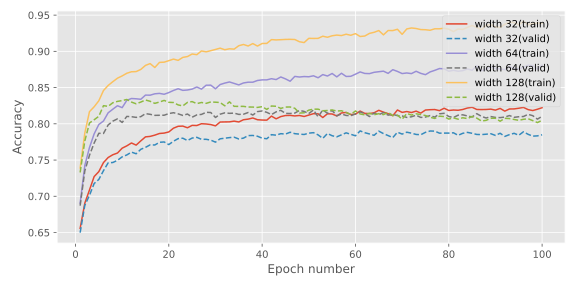
\includegraphics[width=\linewidth]{figures/acc_curve_width.pdf}
        \caption{accuracy by epoch}
        \label{fig:width_acccurves}
    \end{subfigure} 
    \begin{subfigure}{\linewidth}
        \centering
        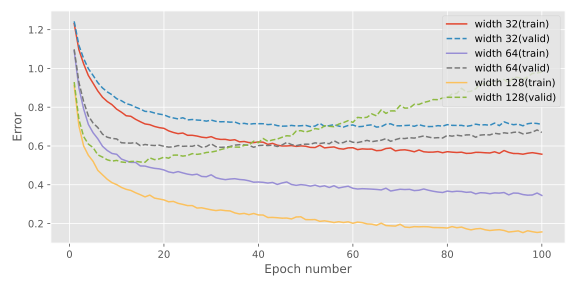
\includegraphics[width=\linewidth]{figures/error_curve_width.pdf}
        \caption{error by epoch}
        \label{fig:width_errorcurves}
    \end{subfigure} 
    \caption{Training and validation curves in terms of classification accuracy (a) and cross-entropy error (b) on the EMNIST dataset for different network widths.}
    \label{fig:width}
\end{figure} 
}
}

%% Question Figure 3:
% Replace these images with figures depicting the accuracy and error, training and validation curves for your experiments varying the number of hidden layers.
\newcommand{\questionFigureThree} {
\youranswer{
\begin{figure}[t]
    \centering
    \begin{subfigure}{\linewidth}
        \includegraphics[width=\linewidth]{figures/acc_curve_depth.pdf}
        \caption{accuracy by epoch}
        \label{fig:depth_acccurves}
    \end{subfigure} 
    \begin{subfigure}{\linewidth}
        \centering
        \includegraphics[width=\linewidth]{figures/error_curve_depth.pdf}
        \caption{error by epoch}
        \label{fig:depth_errorcurves}
    \end{subfigure} 
    \caption{Training and validation curves in terms of classification accuracy (a) and cross-entropy error (b) on the EMNIST dataset for different network depths.}
    \label{fig:depth}
\end{figure} 
}
}

%% Question Figure 4:
\newcommand{\questionFigureFour} {
\youranswer{Question Figure 4 - Replace these images with figures depicting the Validation Accuracy and Generalisation Gap for each of your experiments varying the Dropout inclusion rate, L1/L2 weight penalty, and for the 8 combined experiments (you will have to find a way to best display this information in one subfigure).
%
\begin{figure*}[t]
    \centering
    \begin{subfigure}{.3\linewidth}
        \includegraphics[width=\linewidth]{figures/empty_dropout_plot.png}
        \caption{Metrics by inclusion rate}
        \label{fig:dropoutrates}
    \end{subfigure} 
    \begin{subfigure}{.3\linewidth}
        \centering
        \includegraphics[width=\linewidth]{figures/empty_wd_plot.png}
        \caption{Metrics by weight penalty}
        \label{fig:weightrates}
    \end{subfigure} 
    \begin{subfigure}{.3\linewidth}
        \centering
        \includegraphics[width=.85\linewidth]{example-image-duck}
        \caption{Extra experiments}
        \label{fig:extra}
    \end{subfigure} 
    \caption{Hyperparameter search for every method and combinations}
    \label{fig:hp_search}
\end{figure*}
}
}

%% - - - - - - - - - - - - TABLES - - - - - - - - - - - - 

%% Question Table 1:
\newcommand{\questionTableOne} {
\youranswer{
\begin{table}[t]
    \centering
    \begin{tabular}{c|cc}
    \toprule
        \# hidden units & val. acc. & generalization gap \\
    \midrule
         32            &     0.78       &      0.04              \\
         64            &     0.81       &      0.05              \\
         128           &     0.80       &      0.14              \\
    \bottomrule
    \end{tabular}
    \caption{Validation accuracy (\%) and generalization gap (in terms of cross-entropy error) for varying network widths on the EMNIST dataset.}
    \label{tab:width_exp}
\end{table}
}
}

%% Question Table 2:
\newcommand{\questionTableTwo} {
\youranswer{
\begin{table}[t]
    \centering
    \begin{tabular}{c|cc}
    \toprule
        \# hidden layers & val. acc. & generalization gap \\
    \midrule
         1               & 0.78      & 0.04               \\
         2               & 0.81      & 0.07               \\
         3               & 0.80      & 0.14               \\
    \bottomrule
    \end{tabular}
    \caption{Validation accuracy (\%) and generalization gap (in terms of cross-entropy error) for varying network depths on the EMNIST dataset.}
    \label{tab:depth_exps}
\end{table}
}
}

%% Question Table 3:
% Fill in Table 3 with the results from your experiments varying the hyperparameter values for each of L1 regularisation, L2 regularisation, and Dropout (use the values shown on the table) as well as the results for your experiments combining L1/L2 and Dropout (you will have to pick what combinations of hyperparameter values to test for the combined experiments; each of the combined experiments will need to use Dropout and either L1 or L2 regularisation; run an experiment for each of 8 different combinations). Use \textit{italics} to print the best result per criterion for each set of experiments, and \textbf{bold} for the overall best result per criterion.
%
\newcommand{\questionTableThree} {
\youranswer{
\begin{table*}[t]
    \centering
    \begin{tabular}{c|c|cc}
    \toprule
        Model &  Hyperparameter value(s) & Validation accuracy & Generalisation gap \\
    \midrule
    \midrule
     Baseline &  -                       &               0.836 &              0.290 \\
    \midrule
       \multirow{3}*{Dropout}
              & 0.7                      &               0.840 &     \textit{0.031} \\
              & 0.9                      &      \textit{0.853} &              0.068 \\
              & 0.95                     &               0.844 &              0.092 \\
    \midrule
        \multirow{3}*{L1 penalty}
              & 1e-4                     &      \textit{0.851} &             0.035 \\
              & 1e-3                     &               0.799 &             0.550 \\
              & 1e-1                     &               0.020 &    \textit{0.002} \\
    \midrule
        \multirow{3}*{L2 penalty}  
              & 1e-4                     &               0.832 &             0.106 \\
              & 1e-3                     &      \textit{0.855} &             0.035 \\
              & 1e-1                     &               0.648 &    \textit{-0.01} \\
    \midrule
        \multirow{6}*{Combined}  
              & 0.7, L1 1e-4             &               0.826 &             0.006 \\
              & ?, ?                     &                     &                   \\
              & ?, ?                     &                     &                   \\
              & ?, ?                     &                     &                   \\
              & ?, ?                     &                     &                   \\
              & ?, ?                     &                     &                   \\
    \bottomrule
    \end{tabular}
    \caption{Results of all hyperparameter search experiments. \emph{italics} indicate the best results per series and \textbf{bold} indicate the best overall}
    \label{tab:hp_search}
\end{table*}
}
}

%% END of YOUR ANSWERS
